\section{Numerical simulations}
\label{eq:numerical_simulations}

\subsection{General setup}

We present three numerical tests illustrating planar equivalent layers that intersect a simulated 
magnetic source at the same horizontal plane.
Each test involves defining three versions of a predefined equivalent layer by following three different approaches.
The first approach involves estimating a discrete equivalent layer by solving a linear inverse problem. 
This is the common strategy found in literature.
The second and third approaches estimate discrete layers by numerically evaluating Eq. \ref{eq:p-Fourier}, 
as we explain later in the present section. 
It is important to bear in mind that the first approach is the only one that can be applied to field data.
The equivalent layers obtained by following the second and third approaches depend on the knowledge of
the position, shape and physical-property distribution of the true sources. Consequently, they cannot be 
obtained from field data produced by unknown sources, but only from numerical simulations.
Our objective is to demonstrate that the theoretical framework proposed by 
\cite{oliveirajr_etal2026_1}
for continuous equivalent layers is consistent with the classical space-domain approach, which involves 
solving a linear inverse problem. Here we define the general setup for all tests.

\subsubsection{Synthetic magnetic source}

We have simulated a magnetic source composed of $1241$ horizontally juxtaposed rectangular prisms
(Fig. \ref{fig:Figure2}). 
The prisms extend along the $x$-direction from $\approx -3601$ to $4900$ m and 
along the $y$-direction from $\approx -3000.3$ to $\approx 5800.2$ m. 
Each prism has horizontal side lengths of approximately $256.4$ m in the $x$-direction 
and $204.1$ m in the $y$-direction, with thicknesses ranging from $0$ m to $600$ m. 
The top of the source is delimited by the plane $z^{t}_{0} = 0$ m and varies 
from $0$ to $300$ m, while its bottom ranges from $300$ to $600$ m.
The source has a pseudo-random total-magnetization intensity $\sigma$ 
(Eq. \ref{eq:potential-U-space}) 
varying from $2$ to $3$ A/m according to a uniform distribution and a constant direction defined by the 
unit vector $\hat{\mathbf{v}}$, with inclination $-10.2^{\circ}$ and declination $-19.8^{\circ}$. 
We also consider that the main geomagnetic field has a constant direction given by the unit vector $\hat{\mathbf{u}}$,
with inclination $-30^{\circ}$ and declination $-19^{\circ}$. 

\subsubsection{Synthetic potential fields}

We have set a regular grid of $N_{x} \times N_{y}$ observation points 
$\mathbf{r}^{\dagger}_{i} = (x^{\dagger}_{i}, y^{\dagger}_{i}, z^{\dagger}_{0})^{\top}$, $i \in \{1, \dots, N = N_{x} \, N_{y}\}$,
where $N_{x} = 400$, $N_{y} = 330$. 
The points are located on a planar surface $\mathcal{S}^{\dagger}$ above the magnetic source,
at $z^{\dagger}_{0} = -150$ m.
Figure \ref{fig:Figure3} shows the potential fields produced by the magnetic source at 
the simulated grid of observation points.
The potential fields were computed by using the closed expressions derived by \cite{Nagyetal2000, Nagyetal2002} 
and \cite{Fukushima2020}.
In our three tests, we consider that the observed potential field $d^{o}$ (Eq.  
\ref{eq:observed-data-space}) 
is the approximated total-field anomaly (Fig. \ref{fig:Figure3}a), which means that 
$\alpha_{d} \equiv \alpha(1, \hat{\mathbf{u}}) \, \alpha(1, \hat{\mathbf{v}})$ (Eq. \ref{eq:diff-operators-generic}).

\subsubsection{Equivalent layers layout}

In all tests, we define discrete equivalent layers on the same planar surface $\mathcal{S}''$, 
that intersects the source (Fig. \ref{fig:Figure2}) at $z''_{0} = 200$ m.
All layers are composed of punctual equivalent sources arranged on a regular grid of $N_{x} \times N_{y}$ points 
$\mathbf{r}''_{j} = (x''_{j}, y''_{j}, z''_{0})^{\top}$, $j \in \{1, \dots, M = N_{x} \, N_{y}\}$,
so that each point $\mathbf{r}''_{j}$ is located right below an observation point $\mathbf{r}^{\dagger}_{i}$.

\subsection{Tests}

Each test consists in first specifying the equivalent layer type by setting the operators $\alpha_{a}$ and $D_{a}$ 
via Eq. \ref{eq:diff-operators-generic}.
They act on the scaled inverse distance function $\Psi$ 
(Eq. \ref{eq:Psi}) in the space and Fourier domains,
respectively, to define the elements $a_{ij}$ of the matrix $\mathbf{A}$ 
(Definition \ref{def:discrete-eqlayer}).
The second step of each test is determining three versions of the predefined equivalent layer 
on the planar surface $\mathcal{S}''$ by following three different approaches.

\subsubsection{Approach 1: Classical space-domain equivalent layer}

The first approach involves solving a linear inverse problem to estimate a discrete 
equivalent layer $\mathbf{p}_{\epsilon}$ leading to a predicted data $\mathbf{d}_{\epsilon}$ 
close to the observed data $\mathbf{d}^{o}$ (Definition \ref{def:discrete-eqlayer}).
In this case, the discrete layer is totally defined in the space domain, by following the 
classical approach found in the literature \citep[e.g.,][]{oliveirajr_etal2023}.
Here we apply the method proposed by \cite{takahashi-etal2020, takahashi-etal2022} 
to solve the inverse problem because the spatial configuration of the 
simulated equivalent sources and observation points leads to 
matrices $\mathbf{A}$ (Definition \ref{def:discrete-eqlayer}) having a Block-Toeplitz 
Toeplitz-Block (BTTB) structure.
This method estimates $\mathbf{p}_{\epsilon}$ by using the Conjugate Gradient Least Squares 
(CGLS) algorithm, which naturally imposes some degree of smoothness when run few iterations 
\citep[][p. 166]{aster_etal2019}.
In fact, the discrete layers estimated here were obtained with only $100$ iterations of the 
CGLS method, which is very small compared to the total number of equivalent sources 
($N = 132,000$).

\subsubsection{Approaches 2 and 3: Theoretical closed-form equivalent layers}

The second and third approaches to define a given equivalent layer are developed in the Fourier domain 
and bypass the need to solve a linear inverse problem. Instead, they directly approximate the continuous 
equivalent layer $p_{\varepsilon}$ defined by Eq. \ref{eq:p-Fourier}. 

In both approaches, we compute discrete layers according to the following steps.
We start by computing the pseudogravity anomaly 
(i.e., $\nicefrac{\partial U}{\partial z}$) due to the synthetic source 
at the simulated grid of observation points $\mathbf{r}^{\dagger}_{i}$ located above the synthetic source (Fig. \ref{fig:Figure2}), 
on the planar surface $\mathcal{S}^{\dagger}$ at $z^{\dagger}_{0} = -150$ m.
The pseudogravity anomaly is defined by $k \, \mathcal{F}\left[ U(\mathbf{r}^{\dagger}) \right]$ in the Fourier domain,
where $\mathcal{F}\left[ U(\mathbf{r}^{\dagger}) \right]$ is the Fourier transform of
$U$ (Eq. \ref{eq:potential-U-space}) on the horizontal surface $\mathcal{S}^{\dagger}$.
Then we numerically compute the term $k \, \mathcal{F}\left[ U_{\varepsilon}(\mathbf{r}'') \right]$ (Eq. \ref{eq:p-Fourier}).
The difference between approaches 2 and 3 is the way we numerically compute $\mathcal{F}\left[ U_{\varepsilon}(\mathbf{r}'') \right]$.
In approach 2, we use the Eq. 
\ref{eq:potential-U-epsilon-Fourier-layer-1}, with a given truncating wavenumber $k_{\varepsilon}$. 
In approach 3, the term $\mathcal{F}\left[ U_{\varepsilon}(\mathbf{r}'') \right]$ is computed by using Eq. 
\ref{eq:potential-U-epsilon-Fourier-layer-2}, with a given regularization parameter $\mu_{\varepsilon}$.
In both approaches, we obtain a discrete equivalent layer $\mathbf{p}_{\epsilon}$ (Definition \ref{def:discrete-eqlayer})
in the space domain by numerically evaluating the inverse Fourier transform of Eq. \ref{eq:p-Fourier}, 
using the predefined operators $\alpha_{d}$ and $\alpha_{a}$.

Because the planar equivalent-layer theorem \cite{oliveirajr_etal2026_1} is a nonconstructive 
existence statement 
that does not define how to obtain $k_{\varepsilon}$ or $\mu_{\varepsilon}$ (Eq(s). \ref{eq:potential-U-epsilon-Fourier-layer-1} and 
\ref{eq:potential-U-epsilon-Fourier-layer-2}), we adopt an empirical procedure in our numerical simulations.
In approaches 2 and 3, we actually obtain sets of tentative discrete equivalent layers $\mathbf{p}_{\epsilon}$ (Definition \ref{def:discrete-eqlayer}) 
for different values of $k_{\varepsilon}$ and $\mu_{\varepsilon}$. 
The optima $k_{\varepsilon}$ and $\mu_{\varepsilon}$ are chosen as those that have minimum values 
and produce discrete equivalent layers $\mathbf{p}_{\epsilon}$ that satisfactorily fit the approximated 
total-field anomaly (Fig. \ref{fig:Figure3}a).
We present curves of the data fit against $k_{\varepsilon}$ and $\mu_{\varepsilon}$ 
in the Fig. S1 of the supplementary material.


\subsection{Results}

\subsubsection{Estimated equivalent layers}

Figure \ref{fig:Figure4} shows all estimated equivalent layers obtained in our three tests.
The first, second and third columns of Fig. \ref{fig:Figure4} contain the results obtained 
from each numerical test, while the first, second and third rows of Fig. \ref{fig:Figure4} 
show the results obtained by following approaches 1--3, respectively.
As we can see in Fig. S2 of the supplementary material, the equivalent layers obtained 
in each test, by following different approaches, are very similar to each other.
The differences oscillate around zero and are dominated by short wavelengths.

The layers obtained from our first test (Figures \ref{fig:Figure4}a, d and g) are Neumann's 
equivalent layers \cite{oliveirajr_etal2026_1}, 
were set with $\alpha_{a} = \alpha_{d}$ (Eq. \ref{eq:p-Fourier}) and approximate the
pseudogravity anomaly $\nicefrac{\partial U}{\partial z}$  
due to the synthetic source (Fig. \ref{fig:Figure2}) on the layer plane $\mathcal{S}''$.
As expected, the estimated Neumann's layers have all positive magnetic moment distributions 
with maxima located right above the synthetic source.
The Neumann's layers obtained by following approaches 2 and 3 
(Figures \ref{fig:Figure4}d and g) were defined by using a truncating wavenumber 
$k_{\varepsilon} = 0.020$ (Eq. \ref{eq:potential-U-epsilon-Fourier-layer-1})
and a regularization parameter $\mu_{\varepsilon} = 5.854$ 
(Eq. \ref{eq:potential-U-epsilon-Fourier-layer-2}). 
The $k_{\varepsilon}$ and $\mu_{\varepsilon}$ values were chosen by using the curves shown 
in Figures S1a and d of the supplementary material.

In our second test, we estimate discrete layers (shown in Figures \ref{fig:Figure4}b, e and h) 
with $\alpha_{a} = \left(\mathbf{k}^{\top} \hat{\mathbf{u}} \right) k$ 
(Eq(s). \ref{eq:diff-operators-generic} and \ref{eq:p-Fourier}).
These layers oscillate from negative to positive values and approximate 
the negative magnetic scalar 
potential (i.e., $\nabla U^{\top} \hat{\mathbf{v}}$) due to the synthetic source on the plane $\mathcal{S}''$.
The layers obtained in the second test, by following approaches 2 and 3 
(Figures \ref{fig:Figure4}e and h), were defined by using a truncating wavenumber 
$k_{\varepsilon} = 0.025$ (Eq. \ref{eq:potential-U-epsilon-Fourier-layer-1})
and a regularization parameter $\mu_{\varepsilon} = 1.000$ 
(Eq. \ref{eq:potential-U-epsilon-Fourier-layer-2}). 
The $k_{\varepsilon}$ and $\mu_{\varepsilon}$ values were chosen by using the curves shown 
in Figures S1b and e of the supplementary material.

Figures \ref{fig:Figure4}c, f and i show the discrete equivalent layers estimated in our 
third numerical test, with $\alpha_{a} = \left(\mathbf{k}^{\top} \hat{\mathbf{u}} \right)$ 
(Eq(s). \ref{eq:diff-operators-generic} and \ref{eq:p-Fourier}). 
These layers approximate the $z$ component of the magnetic induction field 
(i.e., $\tfrac{\partial}{\partial z}\nabla U^{\top} \hat{\mathbf{v}}$) due to the 
synthetic source on the layer plane.
Similarly to the layers obtained in the second test (Figures \ref{fig:Figure4}b, e and h), 
the layers obtained in the third test (Figures \ref{fig:Figure4}c, f and i) oscillate from
negative to positive values. 
The main difference is that the latter exhibit significantly shorter wavelength patterns that
are concentrated over the source boundary.
The layers obtained in the third test, by following approaches 2 and 3 
(Figures \ref{fig:Figure4}f and i), were defined by using a truncating wavenumber 
$k_{\varepsilon} = 0.015$ (Eq. \ref{eq:potential-U-epsilon-Fourier-layer-1})
and a regularization parameter $\mu_{\varepsilon} = 49.889$ 
(Eq. \ref{eq:potential-U-epsilon-Fourier-layer-2}). 
The $k_{\varepsilon}$ and $\mu_{\varepsilon}$ values were chosen by using the curves shown 
in Figures S1c and f of the supplementary material.

\subsubsection{Transformed potential fields}

We computed the transformed potential fields $\mathbf{f}_{\epsilon}$ (Eq. \ref{eq:transformed-field-discrete-layer}) 
at the observation points $\mathbf{r}^{\dagger}_{i}$ located on the plane $z^{\dagger}_{0} = -150$ m by using the discrete 
layers obtained from linear inversion (Figures \ref{fig:Figure4}a–c). Figure \ref{fig:Figure5} shows the residuals 
between the potential fields generated by these estimated layers and the synthetic source. The transformed potential 
fields generated by the remaining estimated layers (shown in Figures \ref{fig:Figure4}d–i) are 
similar to those in Fig. \ref{fig:Figure5} and are provided as supplementary material
(Figures S2--S19).

To compute the approximated total-field anomaly and the $x$, $y$ and $z$ components of the magnetic induction field 
due to the Neumann's layers (Figures \ref{fig:Figure4}a, d and g), 
we have used matrices $\mathbf{T}$ (Eq. \ref{eq:transformed-field-discrete-layer}) 
having elements $t_{ij} = \hat{\mathbf{t}}^{\top} \mathbf{H}_{\Psi}(\mathbf{r}^{\dagger}_{i}, \mathbf{r}''_{j}) \, \hat{\mathbf{h}}$,
with unit vectors $\hat{\mathbf{t}}$ equal to, respectively, $\hat{\mathbf{u}}$, $\hat{\mathbf{x}}$, $\hat{\mathbf{y}}$ and
$\hat{\mathbf{z}}$, 
where $\mathbf{H}_{\Psi}$ is the Hessian of function $\Psi(\mathbf{r}^{\dagger}_{i}, \mathbf{r}''_{j})$
(Eq. \ref{eq:Psi}).
To compute the RTP anomaly, we have used a matrix $\mathbf{T}$ 
having elements $t_{ij} = \tfrac{\partial^{2}}{\partial z^{2}} \Psi(\mathbf{r}^{\dagger}_{i}, \mathbf{r}''_{j})$.

The approximated total-field anomaly and $x$, $y$ and $z$ components of the magnetic induction field 
due to the layers shown in Figures \ref{fig:Figure4}b, e and h were computed 
by following the same approach for the Neumann's layer. 
The RTP, however, was computed differently, by following two steps. 
The first step was defined in the space domain and involved multiplying the estimated discrete layer 
by a matrix $\mathbf{T}$ 
having elements $t_{ij} = \tfrac{\partial^{2}}{\partial z^{2}} \Psi(\mathbf{r}^{\dagger}_{i}, \mathbf{r}''_{j})$,
which is the same approach used for the Neumann's layer. 
The resulting transformed field was then numerically convolved with the filter $\nicefrac{k}{\left(\mathbf{k}^{\top} \hat{\mathbf{v}} \right)}$ 
in the Fourier domain, where $\mathbf{v}$ defines the constant magnetization direction of the synthetic source.
This second step is necessary to include the factor $\nicefrac{\alpha_{a}}{\alpha_{d}}$ into the operator 
$\alpha_{t}$ associated with the transformed field (Eq. \ref{eq:alpha-t-generic}).

The estimated discrete layers shown in Fig. \ref{fig:Figure4}c, f and i do not represent the conventional 
equivalent-layer approach applied to magnetic data processing.
Because of that, they lead to potential-field transformations that are not commonly 
found in the literature about equivalent-layer methods.
To compute the approximated total-field anomaly, we use a matrix $\mathbf{T}$ (Eq. \ref{eq:transformed-field-discrete-layer}) 
with elements $t_{ij} = \nabla \Psi(\mathbf{r}^{\dagger}_{i}, \mathbf{r}''_{j})^{\top} \hat{\mathbf{u}}$, 
which represent the directional derivative of first order of $\Psi$ along the constant direction $\hat{\mathbf{u}}$ 
of the simulated main field.
The $x$, $y$ and $z$ components of the magnetic induction field were computed by using matrices $\mathbf{T}$
having elements $t_{ij} = \tfrac{\partial}{\partial x} \Psi(\mathbf{r}^{\dagger}_{i}, \mathbf{r}''_{j})$, 
$t_{ij} = \tfrac{\partial}{\partial y} \Psi(\mathbf{r}^{\dagger}_{i}, \mathbf{r}''_{j})$ and 
$t_{ij} = \tfrac{\partial}{\partial z} \Psi(\mathbf{r}^{\dagger}_{i}, \mathbf{r}''_{j})$, respectively.
To compute the RTP anomaly due to the estimated layers shown in Figures \ref{fig:Figure4}c, f and i, we performed two steps. 
The first step was defined in the space domain and involved multiplying the estimated discrete layer 
by a matrix $\mathbf{T}$ 
having elements $t_{ij} = \tfrac{\partial^{2}}{\partial z^{2}} \Psi(\mathbf{r}^{\dagger}_{i}, \mathbf{r}''_{j})$,
which is the same approach used for the Neumann's layer. 
The resulting transformed field was then numerically convolved with the filter $\nicefrac{1}{\left(\mathbf{k}^{\top} \hat{\mathbf{v}} \right)}$ 
in the Fourier domain, where $\mathbf{v}$ defines the constant magnetization direction of the synthetic source.
This second step is necessary to include the factor $\nicefrac{\alpha_{a}}{\alpha_{d}}$ into the operator 
$\alpha_{t}$ associated with the transformed field (Eq. \ref{eq:alpha-t-generic}).

\subsubsection{Remarks on the numerical results}

There are three key aspects of our results that we would like to highlight.
First, Figures \ref{fig:Figure4} of the present work and Fig. S2 of the supplementary 
material demonstrate that the theoretical framework proposed by \cite{oliveirajr_etal2026_1} 
is compatible with the classical approach for estimating equivalent layers in the space 
domain through the solution of a linear inverse problem.
In particular, the estimated layers obtained from approaches 2 and 3  -- 
by numerically evaluating the inverse Fourier transform of Eq. \ref{eq:p-Fourier} --
are closely aligned with those derived from approach 1, which involves solving a linear inverse problem.

Another important aspect of our results is that all estimated layers (Fig. 
\ref{fig:Figure4}) produce transformed potential fields $\mathbf{f}_{\epsilon}$ (Eq. 
\ref{eq:transformed-field-discrete-layer}) that closely match the fields generated by the 
synthetic source (Fig. \ref{fig:Figure2}), as shown in Fig. \ref{fig:Figure5}. The 
residuals for the RTP anomalies (Figures \ref{fig:Figure5}g, h, and i) exhibit trends along 
the constant magnetization direction of the synthetic source. These trends arise from the 
relatively low inclination $-10.2^{\circ}$ of the synthetic source magnetization.

Finally, our results demonstrate that potential-field transformations can be computed with any 
equivalent layer, provided that $\alpha_{t}$ (Eq. \ref{eq:alpha-t-generic}) is appropriately 
set. This means that the reduction to the pole, for example, is not a transformation that can only 
be computed using the equivalent-layer technique with layers formed by dipoles. Instead, our 
results show that other layers can also be used to estimate the RTP anomaly, as long as $\alpha_{t}$ 
(Eq. \ref{eq:alpha-t-generic}) is properly adjusted, thus confirming the theoretical 
findings of \cite{oliveirajr_etal2026_1}. 
We have shown that when the layer is not formed by dipoles, information about the constant directions 
of the main field and source magnetization is incorporated into $\alpha_{t}$ 
(Eq. \ref{eq:alpha-t-generic}), which the interpreter uses to compute the desired 
potential-field transformation.

\begin{figure}
	\centering
	\noindent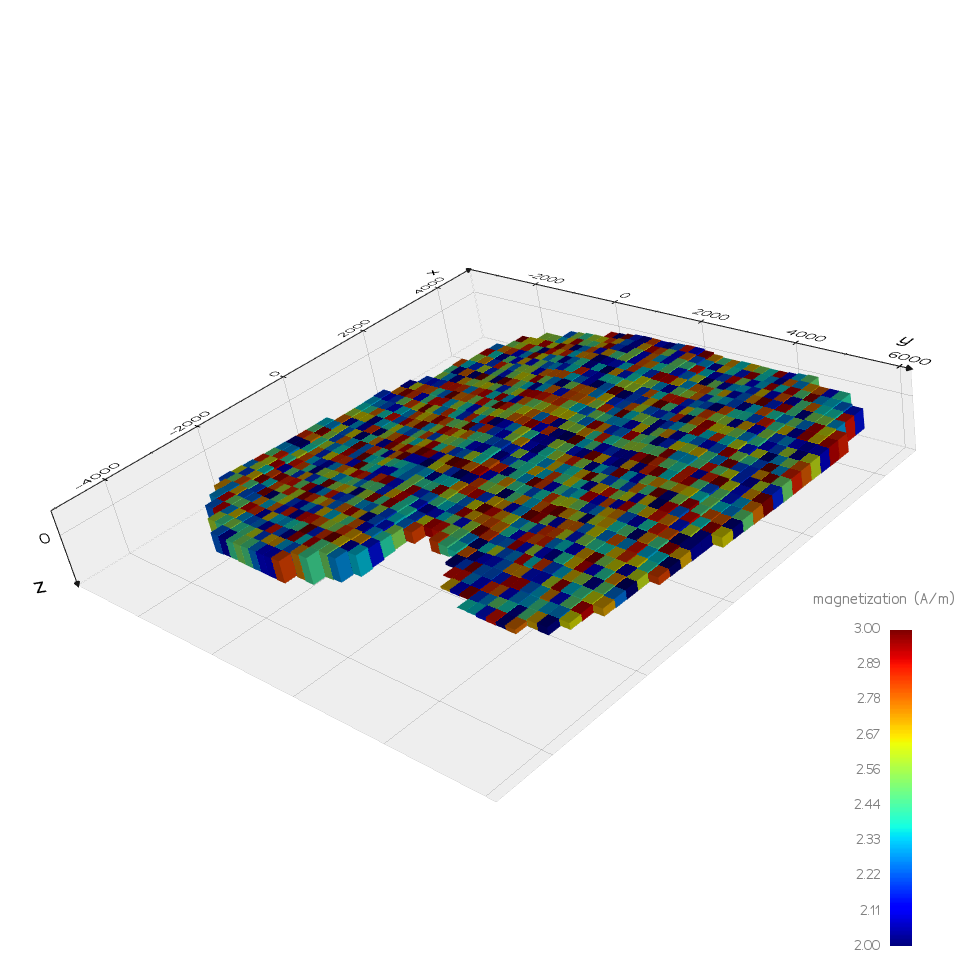
\includegraphics[width=0.8\textwidth]{figures/Figure2_2.png}
	\caption{%
		Simulated magnetic source formed by horizontally juxtaposed rectangular prisms. 
		The model have a pseudo-random total-magnetization intensity $\sigma$  
		varying uniformly from $2$ to $3$ A/m and a constant direction with inclination 
		$-10.2^{\circ}$ and declination $-19.8^{\circ}$.
	}
	\label{fig:Figure2}
\end{figure}

\begin{figure}
	\centering
	\noindent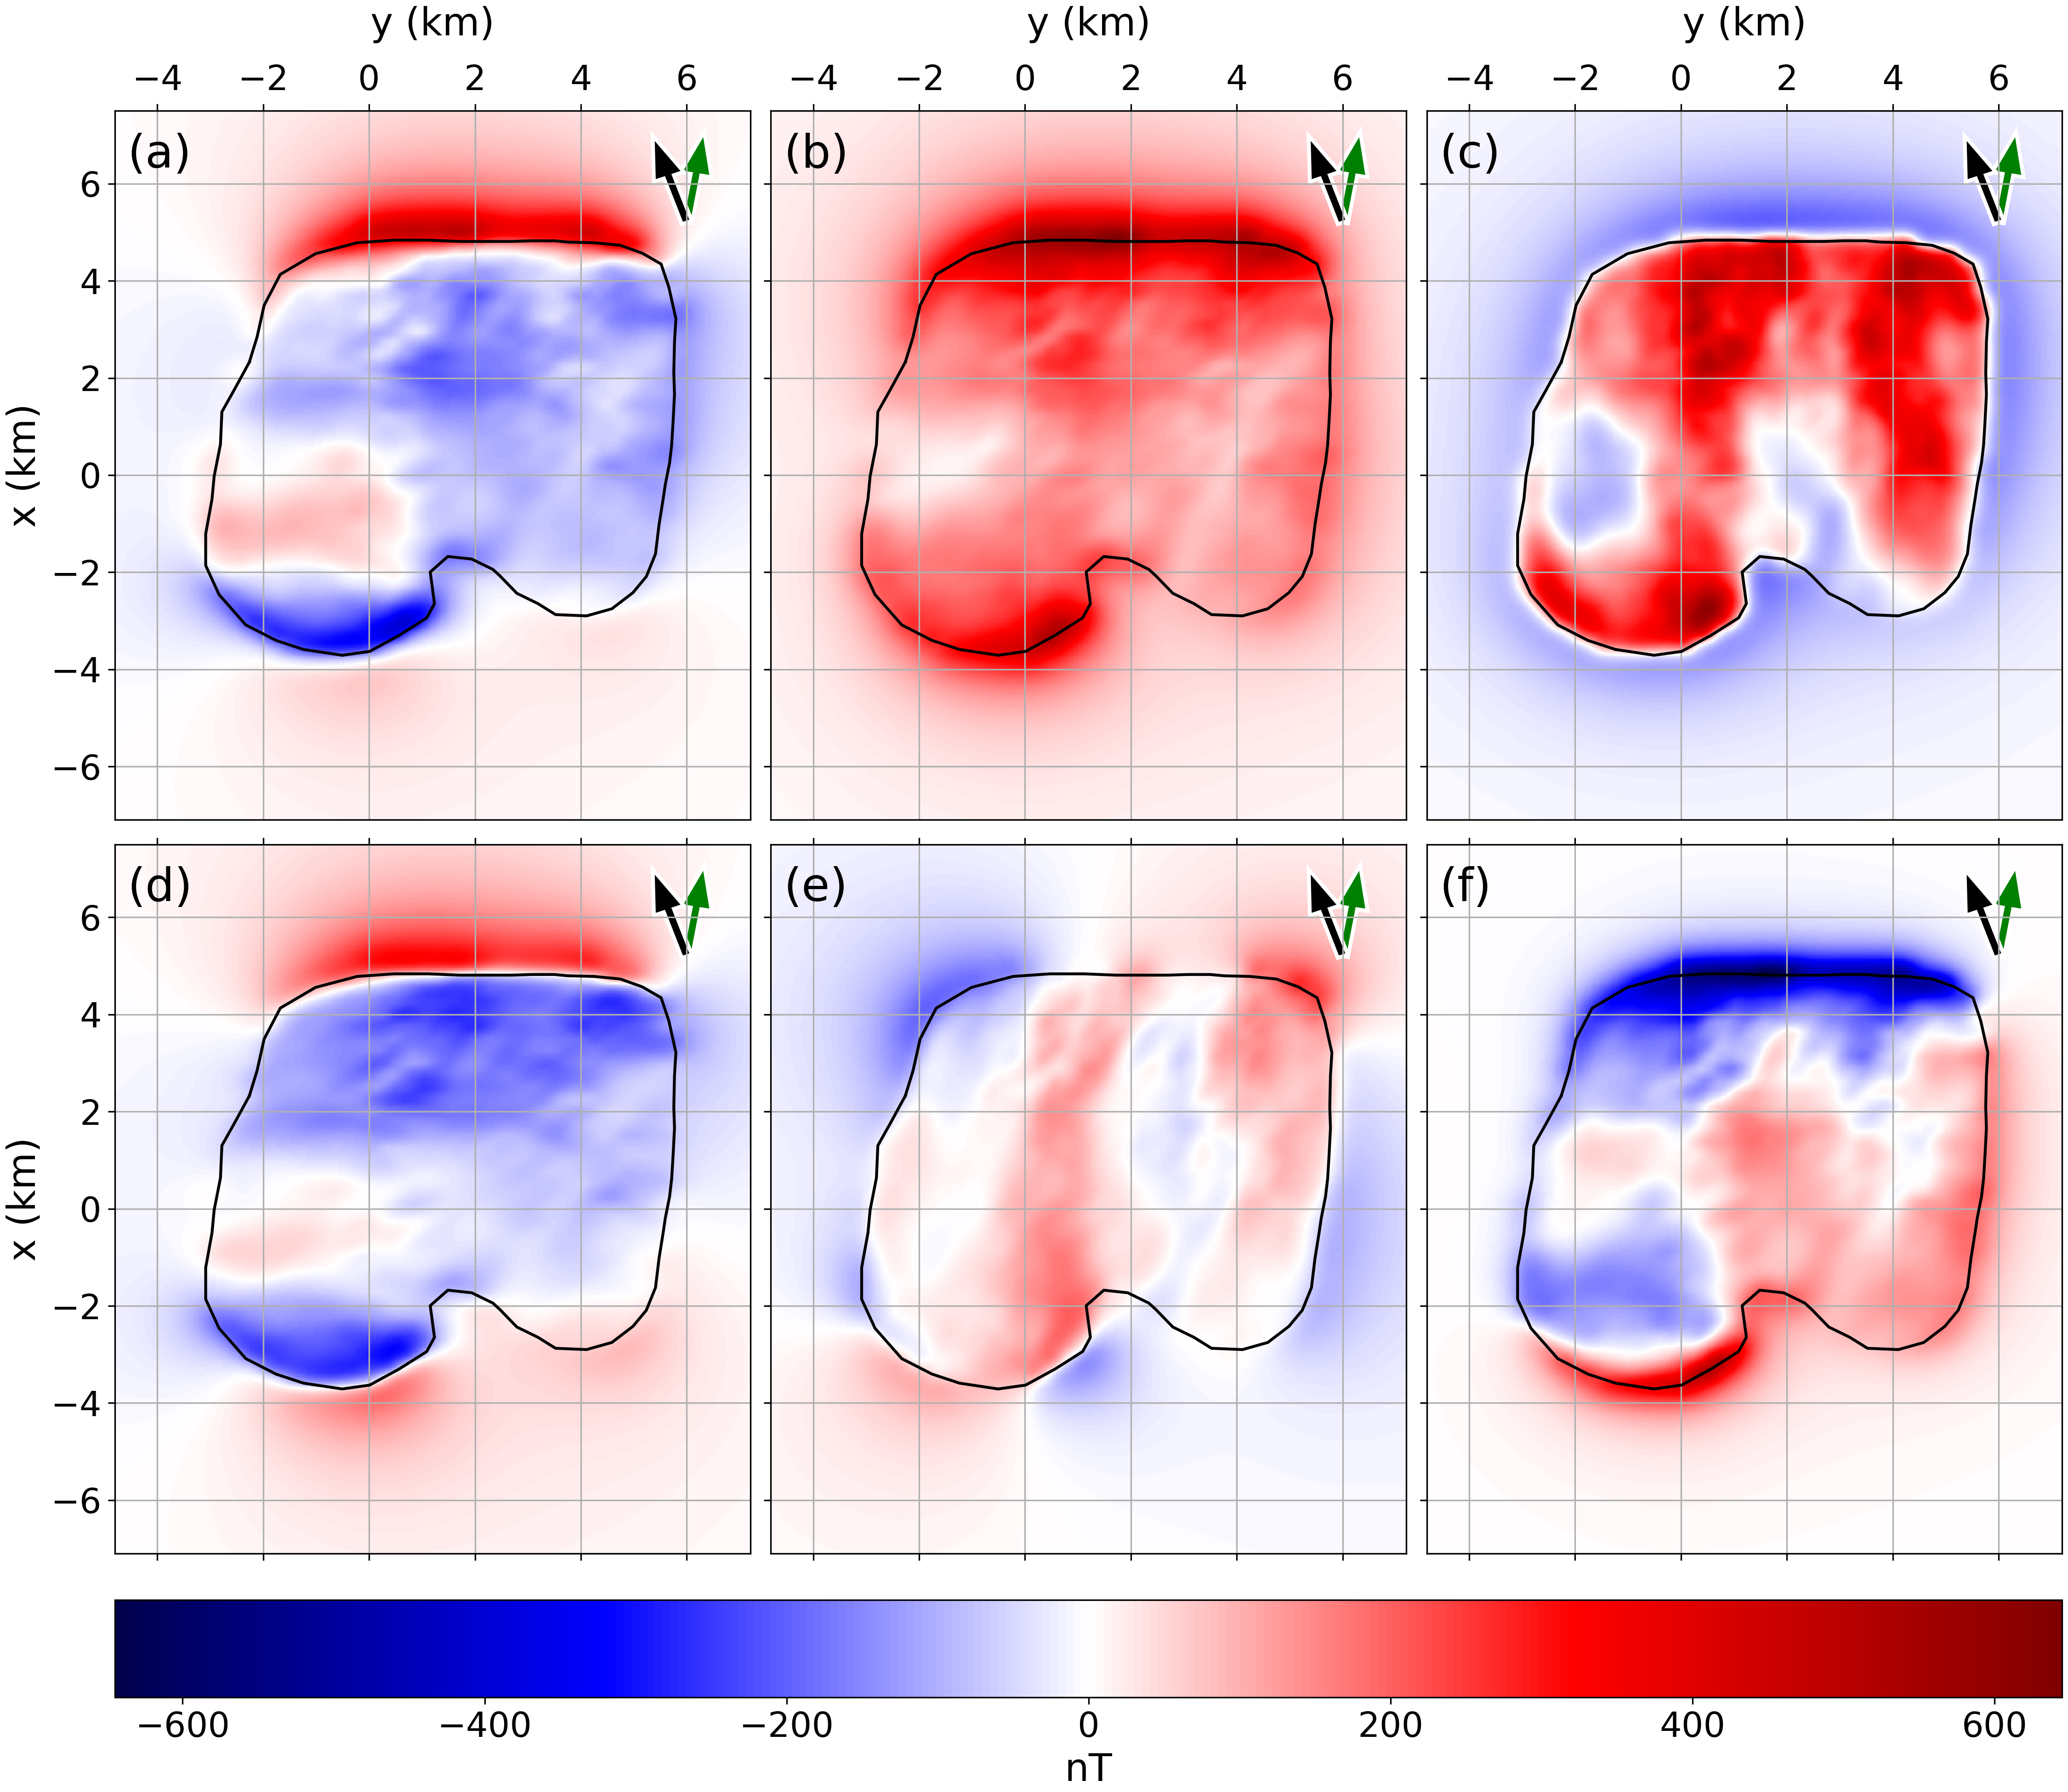
\includegraphics[width=0.8\textwidth]{figures/Figure2_3.png}
	\caption{%
		Potential fields due to the synthetic source (Fig. \ref{fig:Figure2}).
		(a) Approximated total-field anomaly, (b) amplitude of the magnetic induction field, 
		(c) RTP anomaly, (d), (e), (f) $x$, $y$ and $z$ components of the magnetic induction field,
		respectively. All values are in nT.	
		The black line represents the projection of the model on the $xy$ plane.
		The green and black arrows represent, respectively, the projections of the constant 
		main field and synthetic source (Fig. \ref{fig:Figure2}) magnetization directions onto the plane $xy$.
	}
	\label{fig:Figure3}
\end{figure}

\begin{figure}
	\centering
	\noindent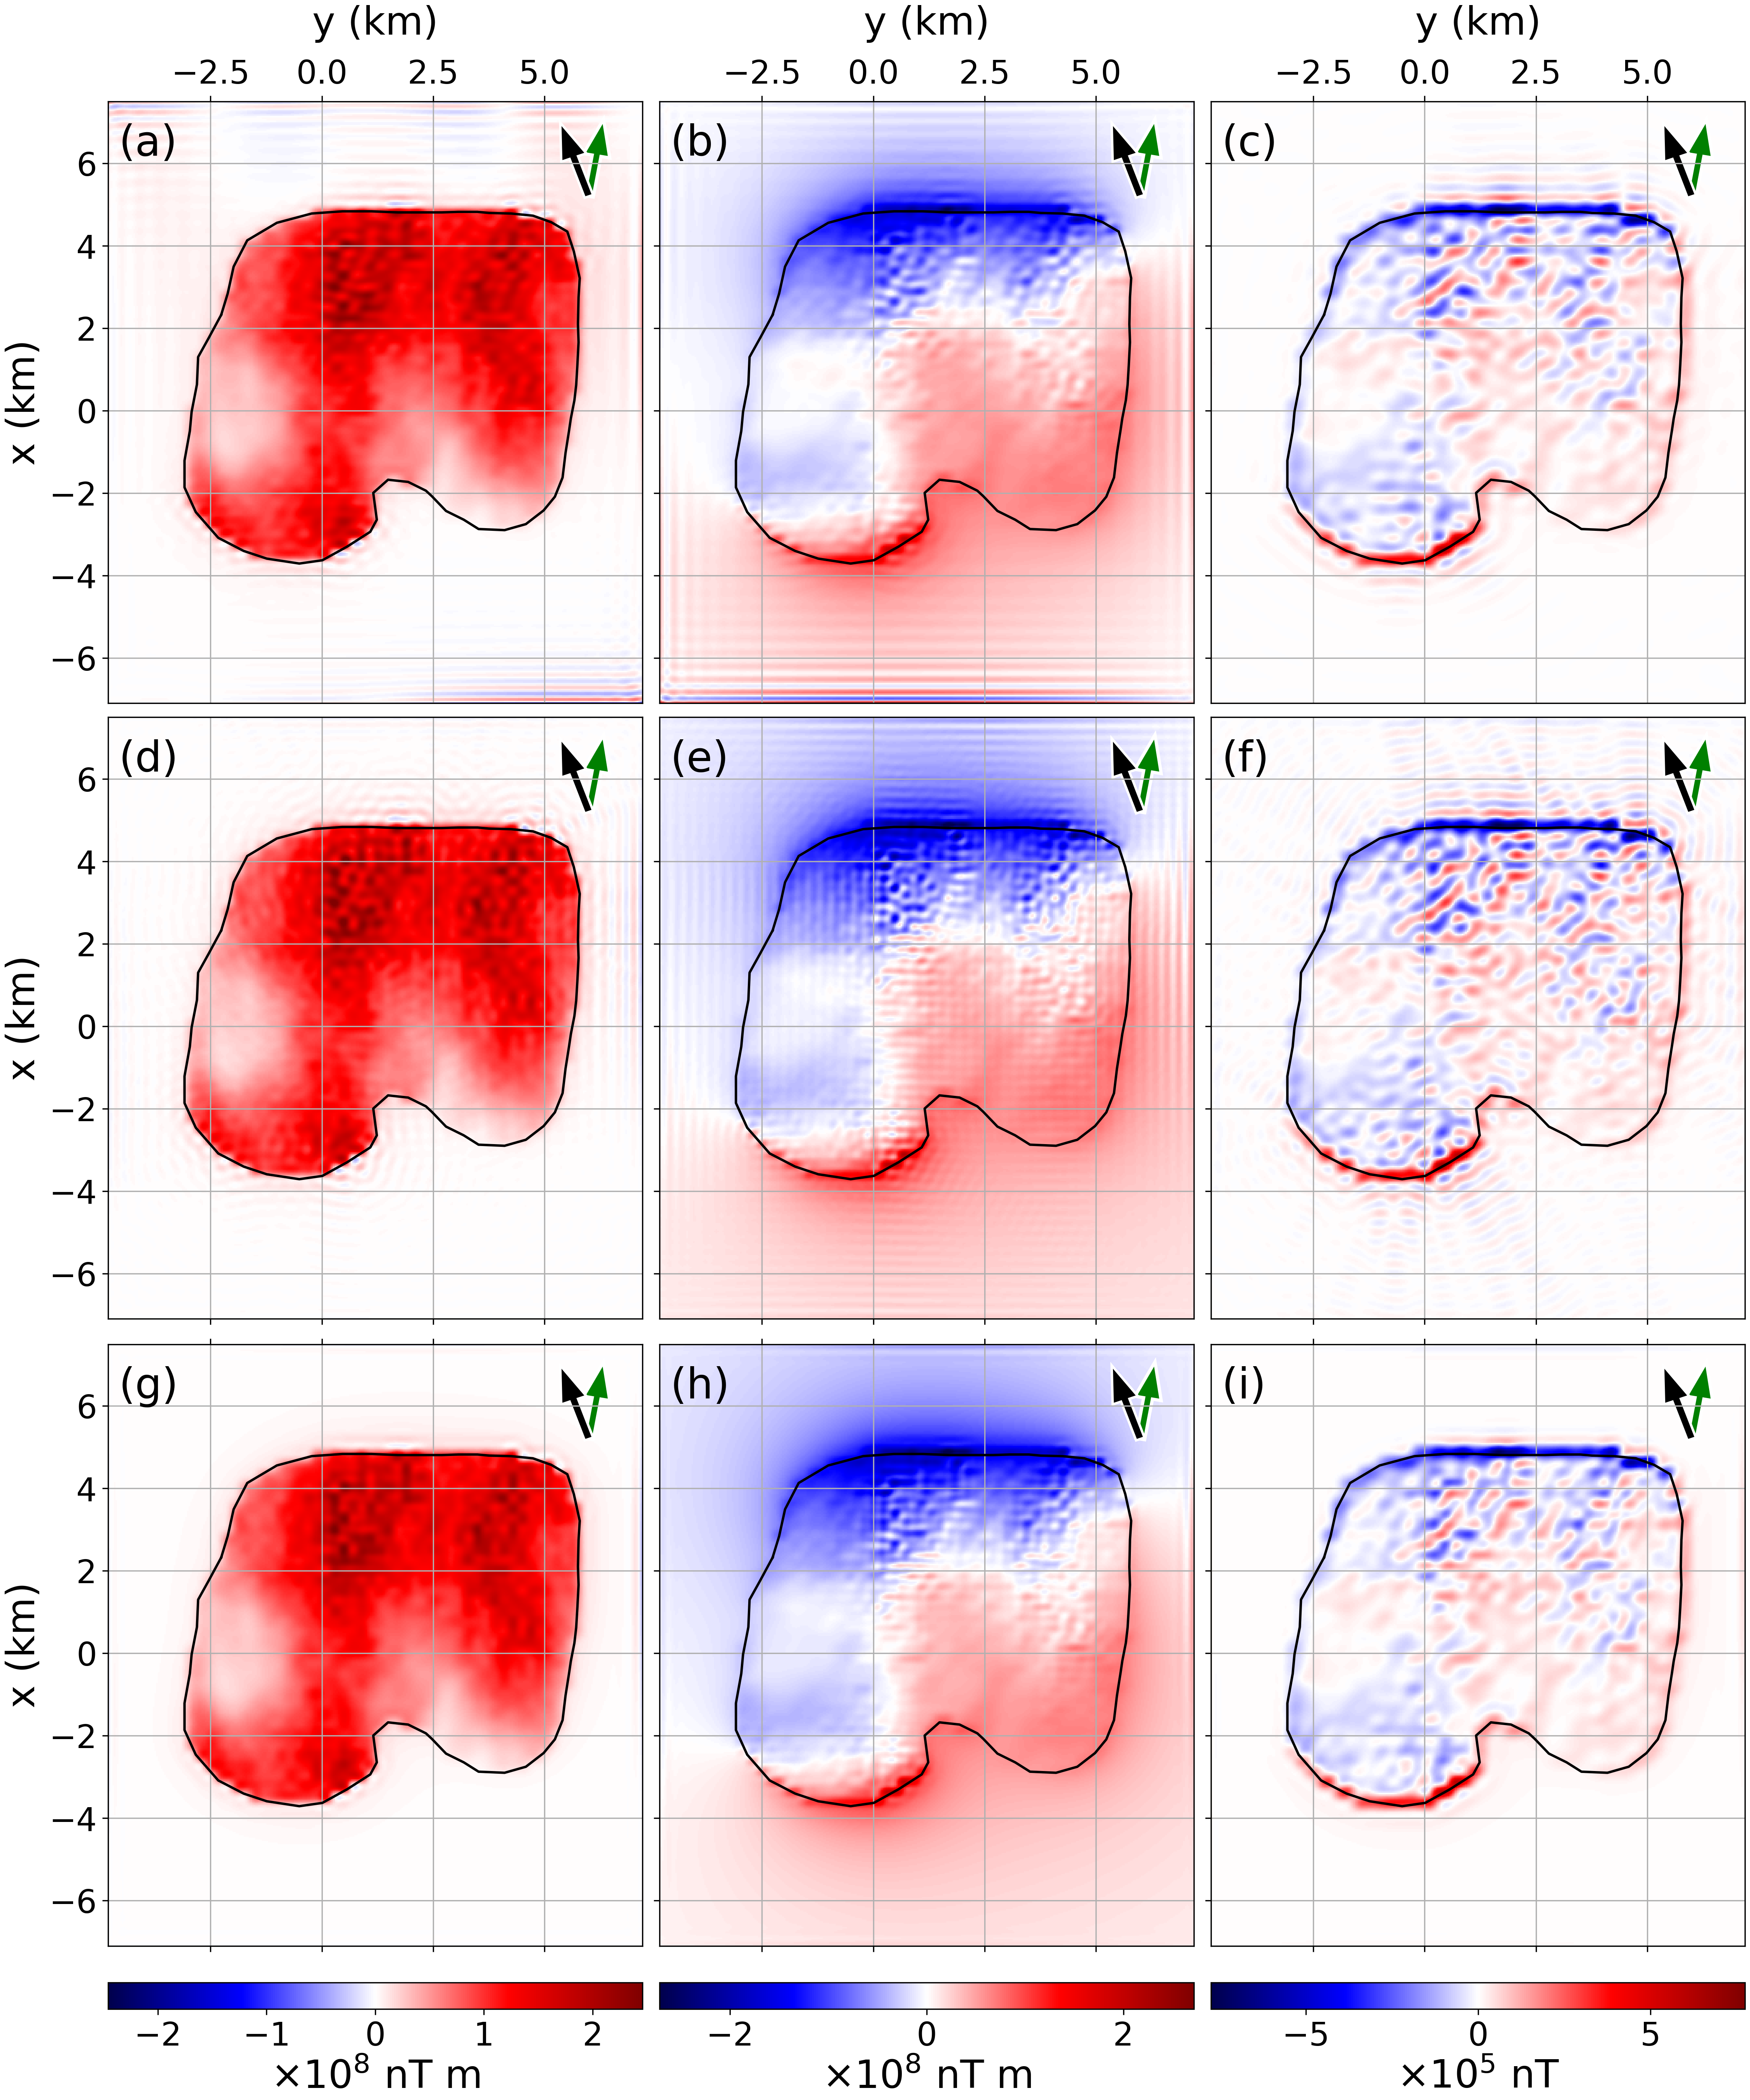
\includegraphics[width=0.8\textwidth]{figures/Figure2_4.png}
	\caption{%
		Estimated discrete layers.
		For all layers, we consider 
		$\alpha_{d} \equiv \alpha(1, \hat{\mathbf{u}}) \, \alpha(1, \hat{\mathbf{v}})$.
		The first, second and third columns contain the results obtained from each numerical test, 
		by using, respectively, $\alpha_{a} = \alpha_{d}$, 
		$\alpha_{a} = \left(\mathbf{k}^{\top} \hat{\mathbf{u}} \right) k$ and 
		$\alpha_{a} = \left(\mathbf{k}^{\top} \hat{\mathbf{u}} \right)$ (Eq. \ref{eq:p-Fourier}). 
		The first, second and third rows show, respectively, the layers estimated by following approaches 1--3.
		The black line represents the projection of the model on the $xy$ plane.
		The green and black arrows represent, respectively, the projections of the constant 
		main field and synthetic source (Fig. \ref{fig:Figure2}) magnetization directions onto the plane $xy$.
	}
	\label{fig:Figure4}
\end{figure}

\begin{figure}
	\centering
	\noindent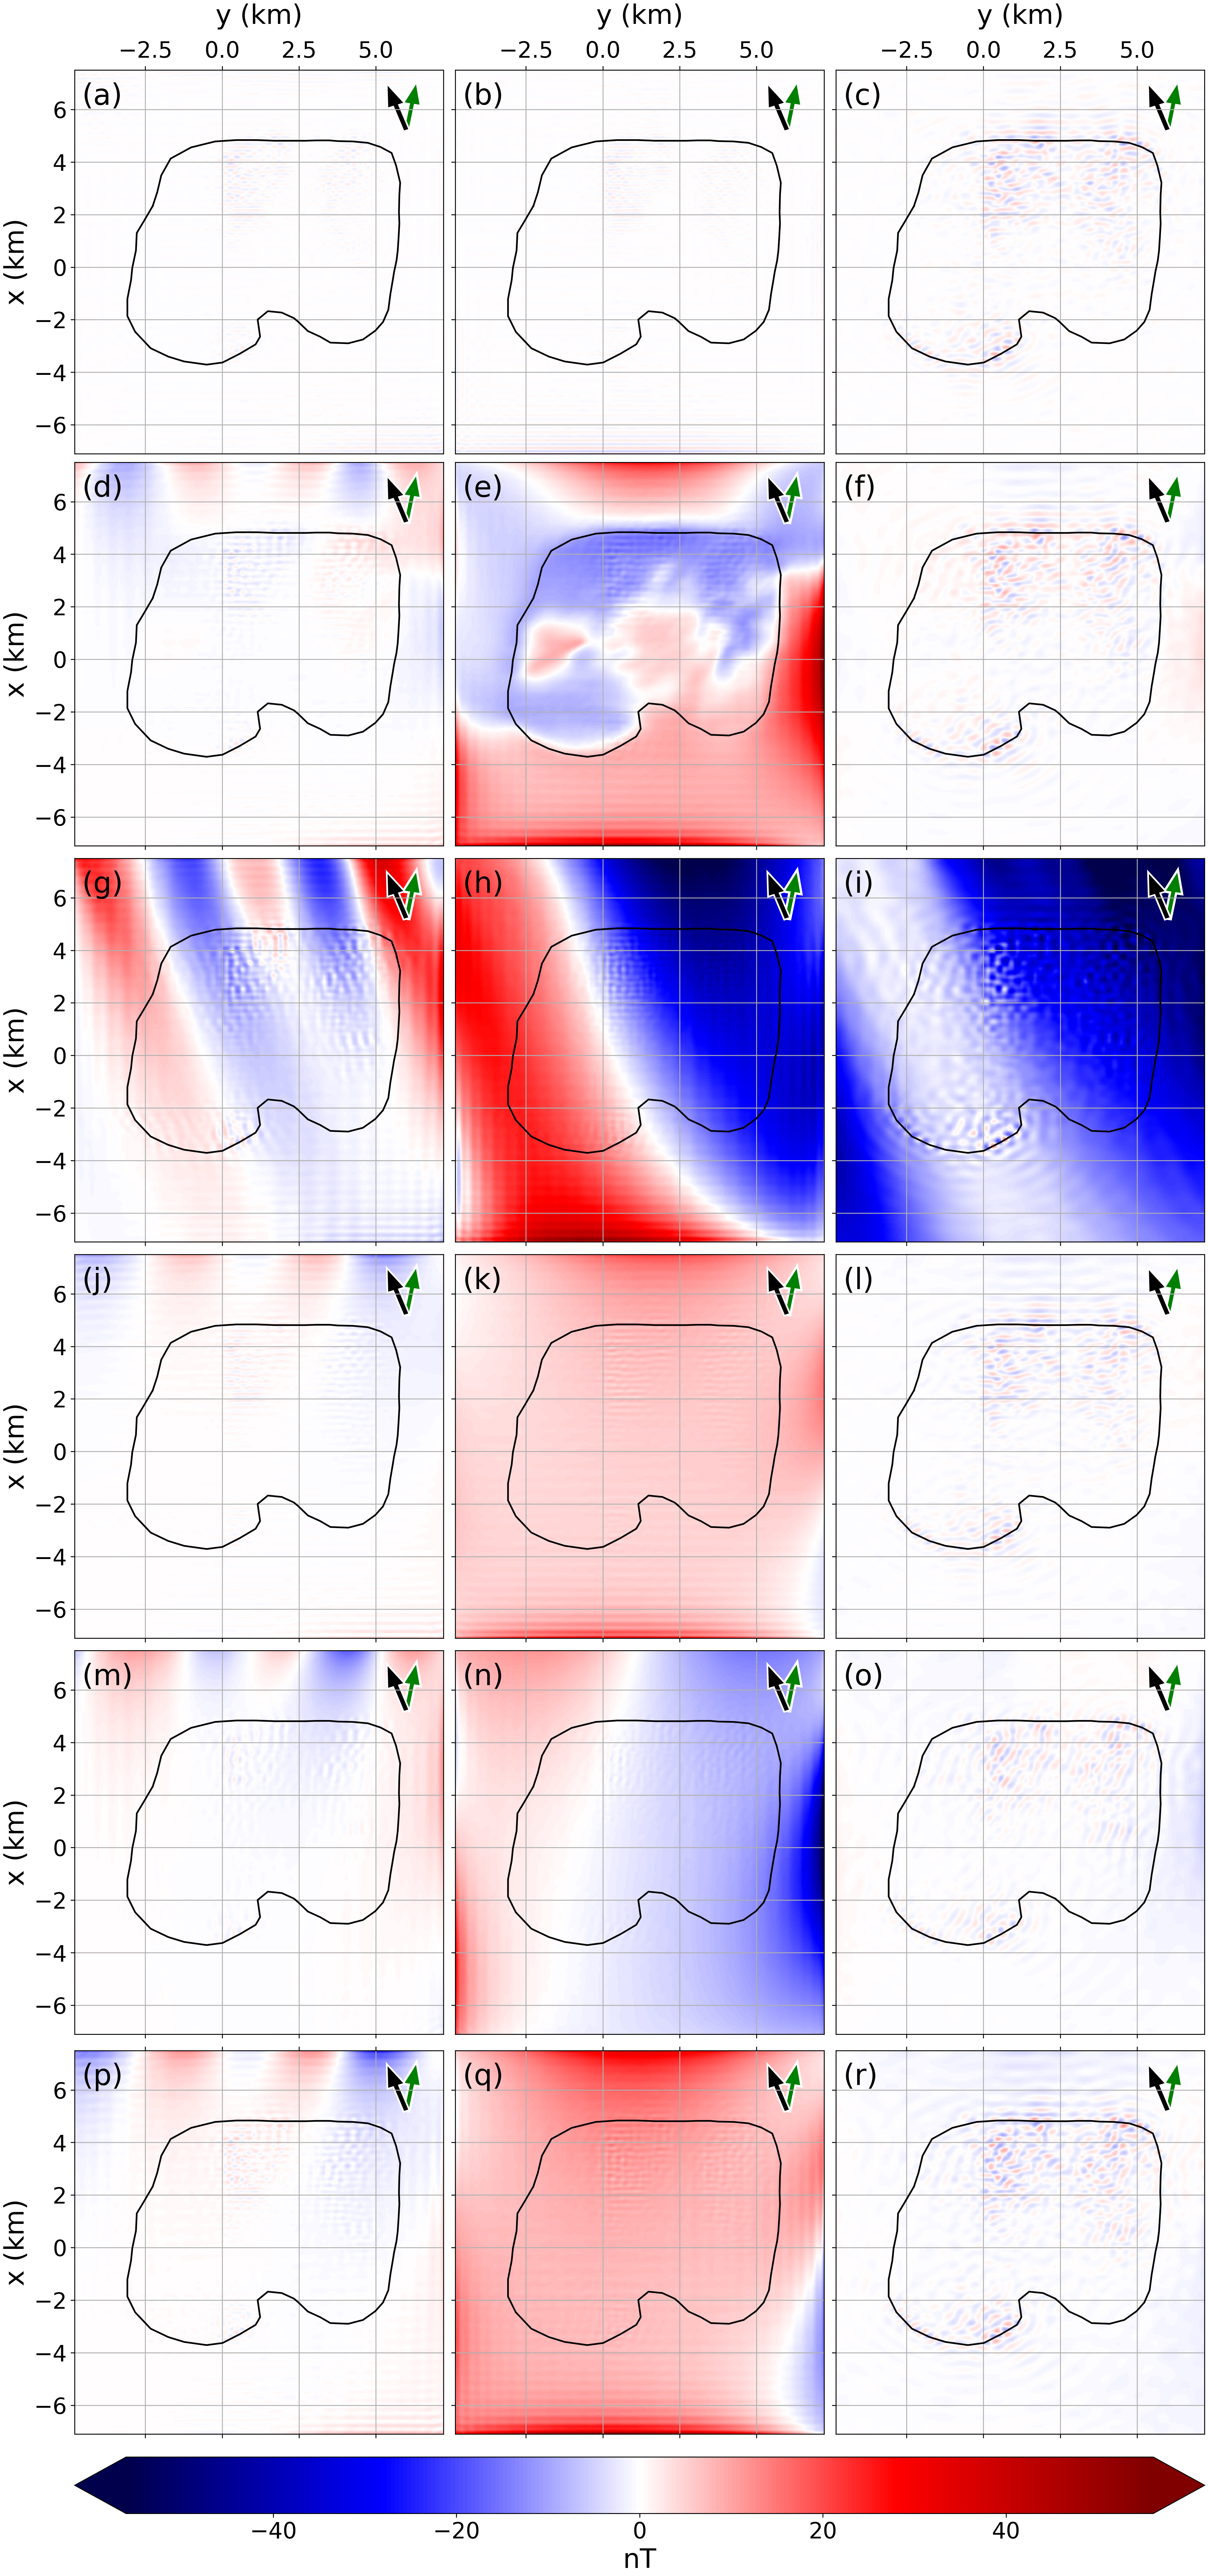
\includegraphics[width=0.65\textwidth]{figures/Figure2_5.png}
	\caption{%
		Residuals between the potential fields due to the synthetic source (Fig. \ref{fig:Figure2}) and
		those produced by the estimated layers shown in Figures \ref{fig:Figure4}a--c.
		The rows from top to bottom contain residuals of the approximated total-field anomaly,
		amplitude of magnetic induction field, RTP anomaly, $x$, $y$ and $z$ components of the magnetic induction field. 
		The columns from left to right contain the potential fields due to the layers shown, respectively, in Figures
		\ref{fig:Figure4}a--c. All values are in nT.
		The black line represents the projection of the model on the $xy$ plane.
		The green and black arrows represent, respectively, the projections of the constant 
		main field and synthetic source (Fig. \ref{fig:Figure2}) magnetization directions onto the plane $xy$.
	}
	\label{fig:Figure5}
\end{figure}